% Рисунки P1. Данные в графиках — из bench/results/ за 2026-08-02.

% --- Рисунок 1: почему разбиение по заполнению страницы даёт перекрытие.
% Одни и те же точки, один и тот же порядок обхода; различается только то, где
% проведены границы страниц. Слева — по заполнению, справа — по picksplit.
\begin{figure}[t]
\centering
\begin{tikzpicture}[scale=1.0,
  pt/.style={circle, fill=black, inner sep=0pt, minimum size=2.6pt},
  key/.style={thick, rounded corners=1pt}]

% Четыре плотных скопления. Координаты заданы явно: на случайных точках
% эффект не читается.
% Четыре плотных скопления. Координаты заданы явно: на случайных точках
% эффект не читается.
\newcommand{\drawpoints}{%
  \foreach \p in {%
    (0.55,2.15),(0.70,2.35),(0.85,2.10),(0.62,2.02),(0.92,2.32),(0.75,2.20),
    (2.25,2.30),(2.45,2.48),(2.60,2.22),(2.32,2.12),(2.58,2.42),(2.44,2.30),
    (0.70,0.80),(0.90,0.98),(1.05,0.72),(0.78,0.65),(1.02,0.95),(0.88,0.82),
    (2.60,0.70),(2.80,0.90),(2.95,0.64),(2.68,0.58),(2.92,0.86),(2.78,0.74)}
    { \node[pt] at \p {}; }%
}

% ---------- (a) разбиение по заполнению страницы
\begin{scope}
  \node[anchor=south, font=\small] at (1.75,3.05) {(a) split by page occupancy};
  \drawpoints
  % порядок обхода ведёт по нижнему ряду, затем по верхнему; страница
  % заполняется до отказа, и граница приходится на середину скопления
  % порядок обхода приводит страницу к концу внутри правого нижнего скопления:
  % его точки достаются обеим страницам, и обе ограничивающие рамки тянутся
  % через всю занятую область
  \draw[key, blue!70!black] (0.45,0.48) rectangle (2.86,2.42);
  \draw[key, red!70!black]  (2.15,0.55) rectangle (3.05,2.58);
  \draw[dashed, gray] (2.78,0.72) circle (0.34);
  \node[font=\scriptsize, blue!70!black, anchor=north west] at (0.0,0.30) {page $i$};
  \node[font=\scriptsize, red!70!black, anchor=north west] at (1.55,0.30) {page $i+1$};
  \node[font=\scriptsize, anchor=north] at (1.75,-0.02) {keys overlap};
\end{scope}

% ---------- (b) разбиение функцией класса операторов
\begin{scope}[xshift=4.6cm]
  \node[anchor=south, font=\small] at (1.75,3.05) {(b) split by \texttt{picksplit}};
  \drawpoints
  \draw[key, blue!70!black] (0.45,1.92) rectangle (2.72,2.58);
  \draw[key, red!70!black]  (0.55,0.45) rectangle (3.05,1.08);
  \node[font=\scriptsize, blue!70!black, anchor=north west] at (0.0,0.30) {page $i$};
  \node[font=\scriptsize, red!70!black, anchor=north west] at (1.55,0.30) {page $i+1$};
  \node[font=\scriptsize, anchor=north] at (1.75,-0.02) {keys disjoint};
\end{scope}
\end{tikzpicture}
\caption{The same entries under the same order; only the choice of page
boundaries differs. Filling each page to capacity (a) puts the boundary in the
middle of a dense region, so the bounding keys of two neighbouring pages cover
almost the same area and a query matching either enters both subtrees.
Delegating the choice to the operator class (b) lets boundaries follow the data
and the keys come out disjoint. Rectangles are the keys stored in the parent.}
\label{fig:split}
\end{figure}

% --- Рисунок 2: перекрытие по уровням не накапливается.
\begin{figure}[t]
\centering
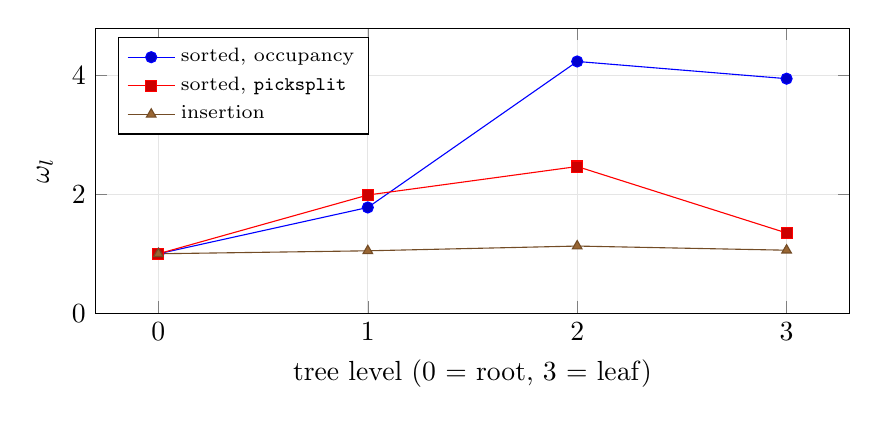
\begin{tikzpicture}
\begin{axis}[
  width=0.92\linewidth, height=5.2cm,
  xlabel={tree level (0 = root, 3 = leaf)},
  ylabel={$\omega_l$},
  xtick={0,1,2,3},
  ymin=0, ymax=4.8,
  legend pos=north west,
  legend style={font=\scriptsize, cells={anchor=west}},
  grid=major, grid style={gray!20},
  mark size=2pt,
]
\addplot+[mark=*] coordinates {(0,1.00) (1,1.78) (2,4.24) (3,3.95)};
\addlegendentry{sorted, occupancy}
\addplot+[mark=square*] coordinates {(0,1.00) (1,1.99) (2,2.47) (3,1.35)};
\addlegendentry{sorted, \texttt{picksplit}}
\addplot+[mark=triangle*] coordinates {(0,1.00) (1,1.05) (2,1.13) (3,1.06)};
\addlegendentry{insertion}
\end{axis}
\end{tikzpicture}
\caption{Overlap per level, $N = 10^7$ uniform points, 2000 probes. Each method
reaches a value characteristic of it within one or two levels of the root and
holds it; overlap does not compound with depth. The upper levels are bounded by
the number of nodes on them.}
\label{fig:levels}
\end{figure}

% --- Рисунок 3: зависимость от размера буфера.
\begin{figure}[t]
\centering
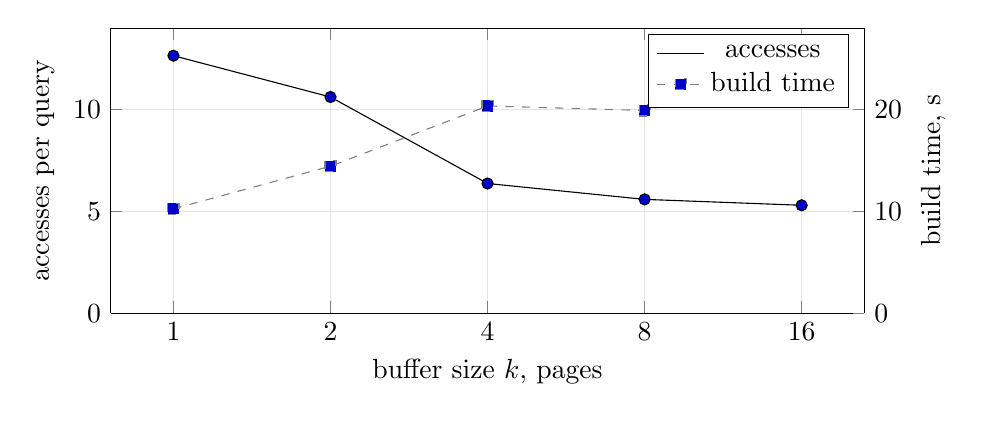
\begin{tikzpicture}
\begin{axis}[
  width=0.92\linewidth, height=5.2cm,
  xlabel={buffer size $k$, pages},
  ylabel={accesses per query},
  xmode=log, log basis x=2,
  xtick={1,2,4,8,16}, xticklabels={1,2,4,8,16},
  ymin=0, ymax=14,
  axis y line*=left,
  grid=major, grid style={gray!20},
  mark size=2pt,
]
\addplot+[mark=*, black] coordinates {(1,12.65) (2,10.62) (4,6.37) (8,5.59) (16,5.30)};
\label{plt:acc}
\end{axis}
\begin{axis}[
  width=0.92\linewidth, height=5.2cm,
  xmode=log, log basis x=2,
  xtick=\empty,
  ylabel={build time, s}, ylabel near ticks,
  ymin=0, ymax=28,
  axis y line*=right, axis x line=none,
  mark size=2pt,
]
\addlegendimage{/pgfplots/refstyle=plt:acc}\addlegendentry{accesses}
\addplot+[mark=square*, gray, dashed] coordinates {(1,10.25) (2,14.44) (4,20.36) (8,19.92) (16,23.58)};
\addlegendentry{build time}
\end{axis}
\end{tikzpicture}
\caption{Dependence on the buffer size, $N = 10^7$ uniform points. $k=1$
reproduces occupancy-based packing. The value shipped in PostgreSQL, $k=4$, is
conservative: $k=8$ improves query cost by 12\,\% at no cost in build time.}
\label{fig:bufsize}
\end{figure}
